\chapter{ARM与嵌入式}

\section{ARM Cortex的指令集}
ARM Cortex主要有9种运行模式,每一种运行模式的代码及说明如下图\nameref{fig:arm_arch}所示
\begin{figure}[H]
  \centering
  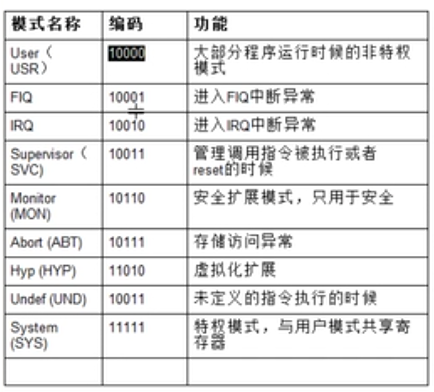
\includegraphics[scale=0.8]{arm_models.png}
  \caption{ARM的运行模式}
  \label{fig:arm_arch}
\end{figure}

ARM还拥有18个寄存器,每个寄存器长度为32位,R0~R12为通用寄存器,R13为栈指针寄存器(SP),R14为
链接指针寄存器(LP),R15为程序计数器(PC),如下图\nameref{fig:arm_reg}所示
\begin{figure}[H]
  \centering
  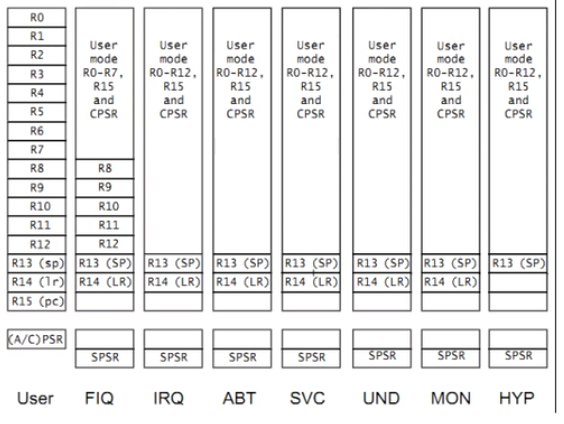
\includegraphics[scale=0.6]{arm_reg.png}
  \caption{ARM寄存器分类}
  \label{fig:arm_reg}
\end{figure}

除了这16个寄存器之外,ARM根据模式的不同,还有APSR(应用程序寄存器)/CPSR(当前程序寄存器)和SPSR(已存储程序寄存器)。
R0-R12寄存器,在所有模式(除快速中断模式)当中共享;快速中断(通常与硬件相关,FIQ)独占R8~R12寄存器;PC和CPSR寄存器是所有模式共享;
其余的寄存器基本是每种模式自己独占;用户模式(Usr)下不存在SPSR。

每一条ARM指令都是32位长度的,CPSR指令的格式大致如下图\nameref{fig:arm_command}所示:
\begin{figure}[H]
  \centering
  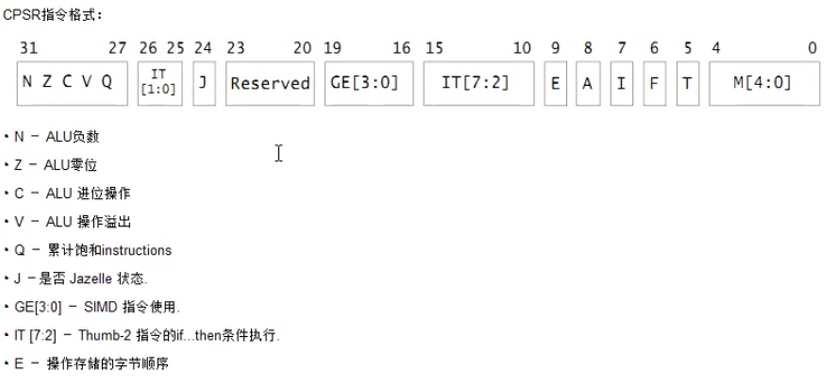
\includegraphics[width=\linewidth]{arm_command.png}
  \caption{ARM指令}
  \label{fig:arm_command}
\end{figure}

其中,指令的最后5位(M[4:0])正好表示本条指令的运行模式;第5位T,表示该指令是否使用是
Thumb指令集,1表示使用;第6位F表示FIQ,表示是否禁用FIQ中断;第7位I表示是否禁用IRQ;
第8位A表示是否禁用异步的abort;第9位E表示操作的字节序,即大小端;10-15位(IT[7:2])表示
Thumb2指令集当中的if-then条件执行;16-19位(GE[3:0])表示SIMD指令(单指令多数据);20-23位
为保留位;24位J表示Jazell状态,是否启用java加速;25-26(IT[1:0])表示Thumb指令集当中的if-then;
27到31分别为Q(累计饱和),V(ALU操作溢出),C(ALU进位操作),Z(ALU零位),N(ALU负数)。

\section{OpenCV交叉编译}
OpenCV是广泛使用的图形图像处理的C/C++函数库,在嵌入式当中,也使用非常广泛。但是,
嵌入式的计算性能毕竟有限,因此,在嵌入式设备上进行OpenCV的编译是非常耗时的。通常采用
交叉编译的方式进行OpenCV的编译,然后再将其移植到ARM等嵌入式设备上,具体操作如下:
\footnote{来源:\url{http://www.studiow.cf/blog/post/how-to-cross-compile-opencv-for-armbian-with-gtk}

\url{https://gist.github.com/Garrus007/6e43211c7a48b4f8600efc6d86d44703}}。

\begin{outline}[enumerate]

\1 安装交叉编译工具链

交叉编译的环境通常在X86的虚拟机或者服务器上,这样能够保证编译的时间。必须注意的是,
由于OpenCV编译完成之后,大多数是so文件,而so文件属于运行时的文件,因此,交叉编译环境
的ldd必须与嵌入式平台的版本一致,否则即使编译完成,也无法进行运行。比较好的做法是,
保持交叉编译环境的操作系统版本和开发板所运行的操作系统版本一致。
\begin{code-in-enumerate}{bash}
apt-get install gcc-arm-linux-gnueabihf g++-arm-linux-gnueabihf \
    pkg-config-arm-linux-gnueabihf -y
\end{code-in-enumerate}

\1 连接嵌入式平台

交叉编译环境上,有很多的类库以及依赖文件,是X86平台上没有或者不匹配的,因此,
我们通过远程连接的方式,将远程的嵌入式平台的操作系统链接到交叉编译环境中。假设
嵌入式平台的ip为172.16.1.155,则操作如下:
\begin{code-in-enumerate}{bash}
sshfs root@172.16.1.155:/ /mnt -o transform_symlinks -o allow_other
\end{code-in-enumerate}

\1 链接嵌入式平台上的开发库以及相关文件

在X86平台上,直接将嵌入式平台上的开发库文件链接到X86本地,方便进行编译开发。
\begin{code-in-enumerate}{bash}
ln -s /mnt/usr/lib/arm-linux-gnueabihf/ /usr/lib/arm-linux-gnueabihf
ln -s /mnt/lib/arm-linux-gnueabihf/ /lib/arm-linux-gnueabihf
ln -s /mnt/usr/share /usr/share/arm-linux-gnueabihf
ln -s /mnt/usr/include/arm-linux-gnueabihf /usr/include/arm-linux-gnueabihf
\end{code-in-enumerate}

注意,由于是通过远程挂载的方式进行交叉编译,因此,需要在嵌入式平台(ARM)上进行
编译所需要的依赖关系的安装。
\begin{code-in-enumerate}{bash}
apt-get install libjpeg-dev libtiff5-dev libjasper-dev libpng12-dev \
    libavcodec-dev libavformat-dev libswscale-dev libv4l-dev \
    libxvidcore-dev libx264-dev libgtk2.0-dev libatlas-base-dev \
    libglib2.0-dev gfortran python2.7-dev python3-dev ffmpeg libgtk-3-dev -y
\end{code-in-enumerate}
当然,如果相关的文件已经安装好了,也可以通过直接复制拷贝的方式,将上面的链接库文件直接拷贝到
交叉编译环境的相对应的路径。

回到X86交叉编译环境,执行下面命令,以上面安装的libgtk2.0-dev为例:
\begin{code-in-enumerate}{bash}
arm-linux-gnueabihf-pkg-config --list-all | grep gtk
arm-linux-gnueabihf-pkg-config --libs gtk+-2.0
arm-linux-gnueabihf-pkg-config --cflags gtk+-2.0
\end{code-in-enumerate}
如果出现下面的显示,则说明交叉编译的依赖关系没有问题了,可以进行编译了。
\begin{figure}[H]
  \centering
  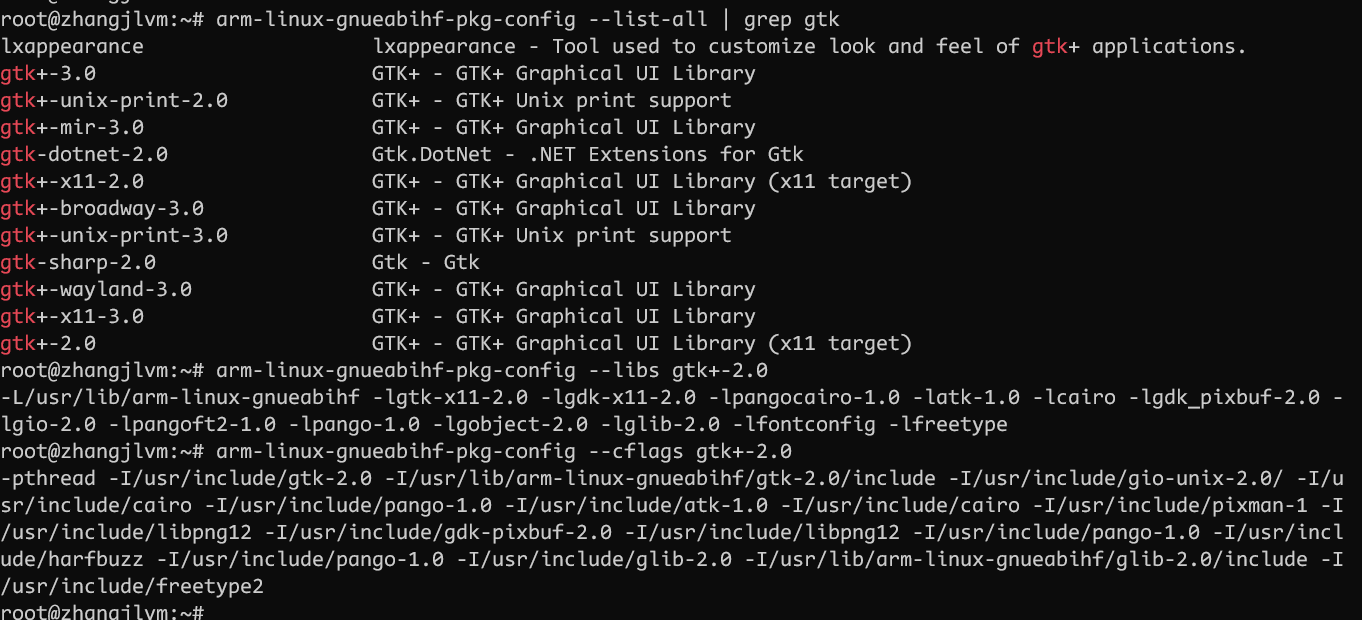
\includegraphics[width=\linewidth]{cross_cv.png}
  \caption{交叉编译的类库}
  \label{fig:cross_cv}
\end{figure}

如果提示错误,则需要按照下面的操作进行:
\begin{code-in-enumerate}{bash}
export PKG_CONFIG_SYSROOT_DIR=/mnt
export PKG_CONFIG_PATH=/usr/share/arm-linux-gnueabihf/pkgconfig:/mnt/usr/lib/pkgconfig
arm-linux-gnueabihf-pkg-config --libs gtk+-2.0
arm-linux-gnueabihf-pkg-config --cflags gtk+-2.0
\end{code-in-enumerate}

\1 下载代码

需要下载OpenCV和OpenCV-Contrib的代码,进行完整编译和模块编译。
\begin{code-in-enumerate}{bash}
git clone https://github.com/opencv/opencv.git
cd opencv && git checkout 3.2.0 && cd
git clone https://github.com/opencv/opencv_contrib.git
cd opencv_contrib && git checkout 3.2.0 && cd ../opencv
\end{code-in-enumerate}

\1 编译代码

首先需要准备编译目录,假设命名为build\_arm
\begin{code-in-enumerate}{bash}
cd opencv
mkdir build_arm
cd build_arm
\end{code-in-enumerate}

修改编译链工具文件
\begin{code-in-enumerate}{bash}
vi ../platforms/linux/arm-gnueabi.toolchain.cmake
\end{code-in-enumerate}

在该文件开始的地方,加入以下的代码:
\begin{code-in-enumerate}{bash}
set(ENV{PKG_CONFIG_PATH} "/usr/share/arm-linux-gnueabihf/pkgconfig:/mnt/usr/lib/pkgconfig")
set(ENV{PKG_CONFIG_SYSROOT_DIR} "/mnt")
set(PKG_CONFIG_EXECUTABLE "/usr/bin/arm-linux-gnueabihf-pkg-config")
set(ENV{LD_LIBRARY_PATH} "/mnt/usr/lib")
set(ENV{C_INCLUDE_PATH} "/mnt/usr/include")
set(ENV{CPLUS_INCLUDE_PATH} "/mnt/usr/include")
\end{code-in-enumerate}

OpenCV3.2.0版本的分支还存在一个小小的bug,需要手动修复一下,否则会影响交叉编译。
修改opencv\_contrib/modules/freetype/CMakeLists.txt,将第22行修改为如下内容:
\footnote{来源:\url{https://github.com/opencv/opencv_contrib/pull/926}}。
\begin{code-in-enumerate}{bash}
ocv_define_module(freetype opencv_core opencv_imgproc PRIVATE_REQUIRED ${FREETYPE_LIBRARIES} ${HARFBUZZ_LIBRARIES} WRAP python)
\end{code-in-enumerate}

然后生成makefile文件:
\begin{code-in-enumerate}{bash}
cmake -DENABLE_NEON=ON -DENABLE_VFPV3=ON  -D WITH_V4L=ON  -D WITH_GTK=ON \
    -D CMAKE_BUILD_TYPE=Release -D BUILD_TESTS=OFF \
    -D CMAKE_TOOLCHAIN_FILE=/root/opencv/platforms/linux/arm-gnueabi.toolchain.cmake \
    /root/opencv/ -D OPENCV_EXTRA_MODULES_PATH=/root/opencv_contrib/modules ..
\end{code-in-enumerate}

如果cmake的信息当中,提示GUI没有支持,一定要在嵌入式平台端安装GTK或者QT等图形化开发
的lib库,否则,OpenCV在运行时,将无法显示图像。
\begin{figure}[H]
  \centering
  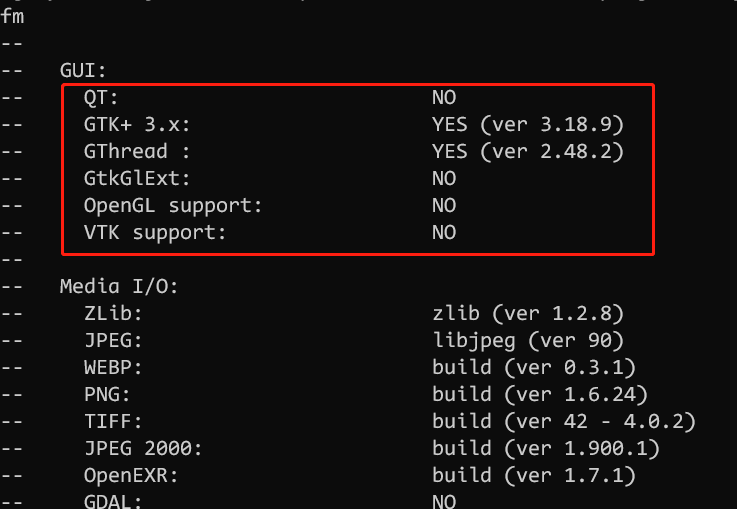
\includegraphics[scale=0.3]{cross_gui.png}
  \caption{图形化支持}
  \label{fig:cross_gui}
\end{figure}

随后进行OpenCV的编译:
\begin{code-in-enumerate}{bash}
make
make install
\end{code-in-enumerate}
如果一切顺利,将在opencv/build\_arm/install生成我们所需要的OpenCV文件,包括头文件,
so文件和其他的文件,大致如下:
\begin{figure}[H]
  \centering
  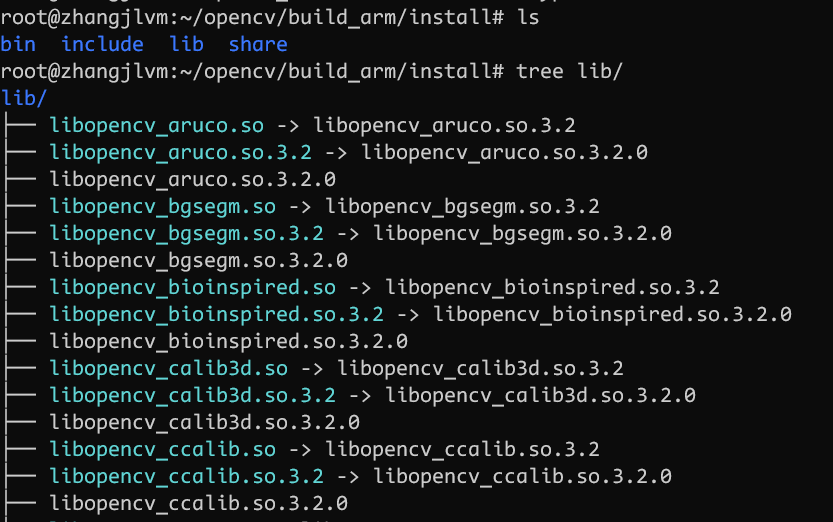
\includegraphics[width=\linewidth]{cross_finish.png}
  \caption{交叉编译的结果}
  \label{fig:cross_finish}
\end{figure}

然后将install下的所有文件,放到嵌入式系统的/usr/local当中对应的目录即可,注意,需要
修改install/lib/pkgconfig/opencv.pc文件,将prefix修改,修改为如下:
\begin{code-in-enumerate}{bash}
prefix=/usr/local
\end{code-in-enumerate}

断开交叉编译环境与嵌入式系统的文件链接:
\begin{code-in-enumerate}{bash}
fusermount -u /mnt
\end{code-in-enumerate}

完成上述操作之后,在嵌入式系统当中,执行指令:
\begin{code-in-enumerate}{bash}
ldconfig -v
\end{code-in-enumerate}

如果输出结果类似下面,则说明编译OpenCV移植成功,则ARM的嵌入式系统当中,可以正常使用。
\begin{figure}[H]
  \centering
  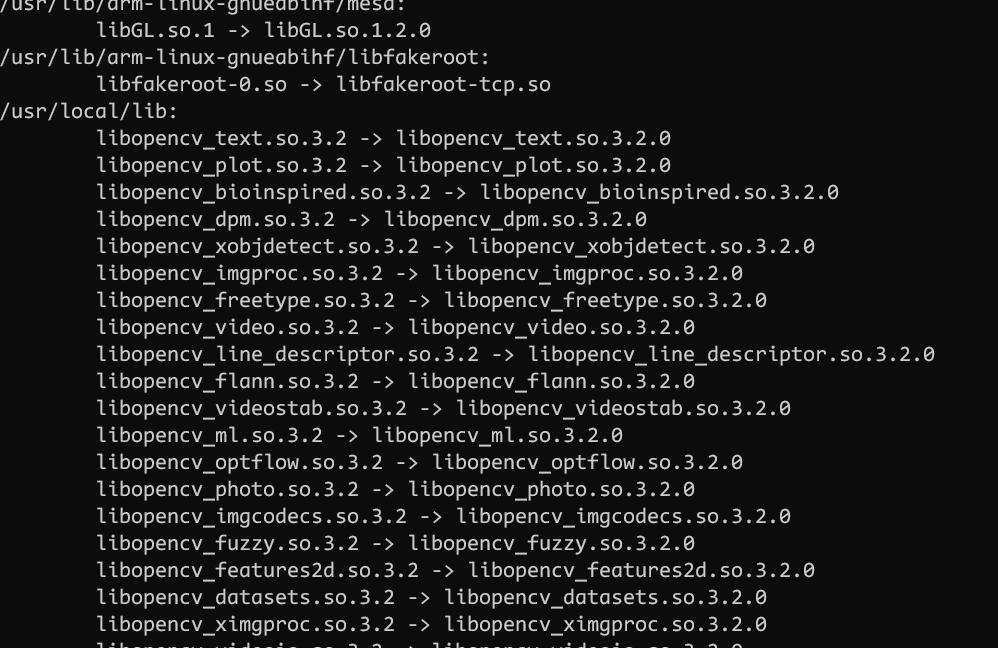
\includegraphics[width=\linewidth]{cross_transplant.png}
  \caption{移植到嵌入式系统}
  \label{fig:cross_transplant}
\end{figure}

\1 测试功能

移植之后,需要调用OpenCV的函数,才知道最终的结果。为此,我们编写一个简易的OpenCV应用程序,
只要能够将图片显示出来,就基本表明OpenCV的移植是没有问题的了。

代码的功能比较简单,就是读取一张图片,并显示出来,具体的代码如下:
\begin{code-in-enumerate}{cpp}
#include <opencv2/opencv.hpp>

using namespace cv;

int main(void)
{
        Mat img, gray;
        img = imread("lena.bmp", CV_LOAD_IMAGE_COLOR);
        imwrite("show", img);
        waitKey(0);
        destroyAllWindows();
        return 0;
}
\end{code-in-enumerate}

使用编译指令进行编译:
\begin{code-in-enumerate}{bash}
g++ -std=c++11 -Wall `pkg-config --cflags opencv` \
    -o canny canny.cc  `pkg-config --libs opencv` -lpthread
\end{code-in-enumerate}

也可以使用Makefile:
\begin{code-in-enumerate}{make}
TARGET = canny

CFLAGS = -Ofast -Wall -std=c++11 `pkg-config --cflags opencv`
LDFLAGS = -Ofast -Wall -std=c++11 `pkg-config --libs opencv`
CC = g++

all: $(TARGET)

$(TARGET): $(TARGET).o
        $(CC) $(LDFLAGS) -o $@ $^ `pkg-config --libs opencv` -lpthread

%.o: %.cpp
        $(CC) $(CFLAGS) -c -o $@ $<

clean:
        rm -f $(TARGET) *.a *.o *~
\end{code-in-enumerate}

执行该代码,如果该代码正常运行,且将图片正常显示,则表明OpenCV的移植没有任何
问题了,整个移植过程成功了。

\end{outline}
